%!TEX TS-program = xelatex  
%!TEX encoding = UTF-8 Unicode  
\documentclass[a4paper, 11pt]{article}
\usepackage{ctex}
\usepackage[margin=1in]{geometry}
\setmainfont{HiraginoSansGB-W3}
\setCJKmainfont{HiraginoSansGB-W3}
\setCJKsansfont{HiraginoSansGB-W3}

\usepackage{graphicx}
\usepackage{subfigure}
\usepackage{hyperref}
\usepackage{listings}
\lstset{language=C++} 

\begin{document}

\title{Badkid: ELF文件病毒设计报告}

\author{柯嵩宇\\ 5140309567 \and 陈天垚 \\ 5140309566 \and 万诚 \\ 5140309552  \and 杨闰哲\\ 5140309562	 \vspace{1em}}
\maketitle

这篇文档的目的,在于还原我们小组对我们的ELF文件病毒“badkid”的设计过程,以及我们在整个设计过程中的技术思考。但请原谅,我们不会在此文中专门介绍ELF文件格式等网上随处可搜到的内容,而是力图忠实地记录我们在实现设计目标中“走过的弯路”与“乍现的灵光”,希望以此给那些想要亲自动手写一个ELF文件病毒(或是想要对抗此类病毒)读者,带来一些有益的启发。

\tableofcontents
\newpage
\section{项目简介}
	此项目中,我们的目的是设计一个感染ELF文件的寄生病毒:当一个ELF文件被其感染时,会修改它的程序入口(entry point);当用户运行一个被感染文件时,就会先执行病毒代码,感染同目录下的其他文件,从而达到复制与传播的效果。宿主程序的执行顺序如图\ref{fig:order}所示。
	\vspace{1em}
	\begin{figure*}[htbp]
		\centering
		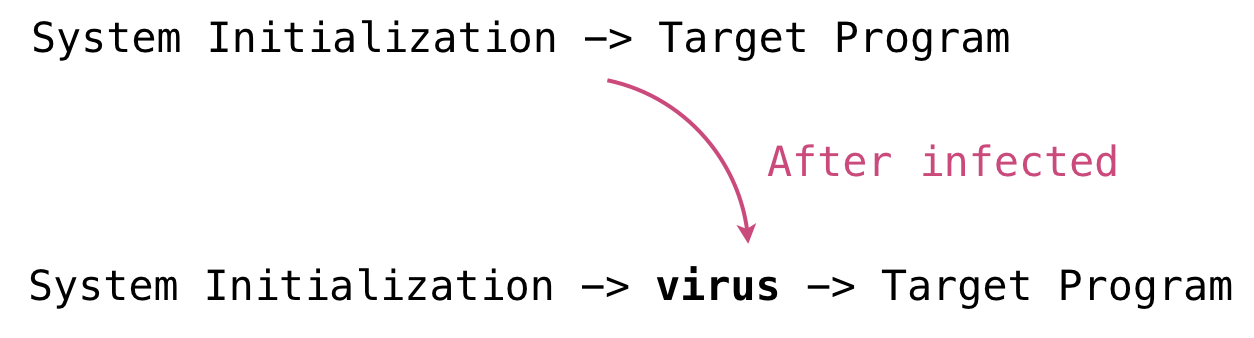
\includegraphics[width = \textwidth]{figures/fig3_first}
		\caption{受感染寄主程序的执行顺序}
		\label{fig:order}
	\end{figure*}
\subsection{重要假设}	
	我们假定病毒工作于以下环境:
	\begin{enumerate}
		\item 指令集架构:x86\_64
		\item 操作系统:Linux\footnote{实际环境为Ubuntu 16.04 x86\_64 LTS}
		\item 病毒母体能够以\texttt{root}权限执行
	\end{enumerate}
	
	因为假设了病毒在执行时有root权限,这样我们可以专注于ELF文件的分析与重构、病毒的攻击行以及病毒本身,而不用操心其他问题。
\section{技术背景}
\subsection{Linux系统}
Linux是一种自由和开放源代码的类UNIX操作系统。该操作系统的内核由林纳斯·托瓦兹在1991年10月5日首次发布。在加上用户空间的应用程序之后,成为Linux操作系统。

Linux最初是作为支持英特尔x86架构的个人电脑的一个自由操作系统。目前Linux已经被移植到更多的计算机硬件平台,远远超出其他任何操作系统。Linux可以运行在服务器和其他大型平台之上,如大型主机和超级计算机。世界上500个最快的超级计算机90%以上运行Linux发行版或变种,包括最快的前10名超级电脑运行的都是基于Linux内核的操作系统。Linux也广泛应用在嵌入式系统上,如手机(Mobile Phone)、平板电脑(Tablet)、路由器(Router)、电视(TV)和电子游戏机等。在移动设备上广泛使用的Android操作系统就是创建在Linux内核之上。\footnote{来自维基百科}
\subsection{Executable and Linkable Format(ELF)}
可执行和可链接格式常被称为ELF格式,在计算机科学中,是一种用于可执行文件、目标文件、共享库和核心转储的标准文件格式。

1999年,被86open项目选为x86架构上的类Unix操作系统的二进制文件格式标准,用来取代COFF。因其可扩展性与灵活性,也可应用在其它处理器、计算机系统架构的操作系统上。
\section{四个思路}
设计一个ELF病毒的核心问题是,如何寄生我们的ELF病毒。如果我们直接让病毒直接覆盖宿主,受感染后的宿主文件被破坏,即让它覆盖可执行文件,破坏原始数据。这种传染方式将导致下次宿主程序执行失败,病毒很易被发现。如果被破坏的宿主是系统赖以生存的重要文件,将导致整个系统崩溃。我们更希望在向宿主文件中插入病毒体时,不破坏宿主主体,修改程序流程,以便病毒跟随宿主一起执行。这种情况下寄生病毒不改变宿主内部对象格式,在自身得到执行后将控制交还给宿主。但是如何把病毒体嵌入宿主文件中呢,我们做了一下尝试。
\subsection{静态链接病毒}
最开始的想法是用静态链接编译我们的病毒。如果把自己的代码编译成静态的,这样在嵌入文件的时候就不需要考虑载入外部文件时的问题,只需要修改一些位置就可以执行代码了。如:ELF的\texttt{EntryPoint},\texttt{\_start()}函数中\texttt{\_\_libc\_start\_main}函数的参数等。
	\begin{figure*}[htbp]
		\centering
		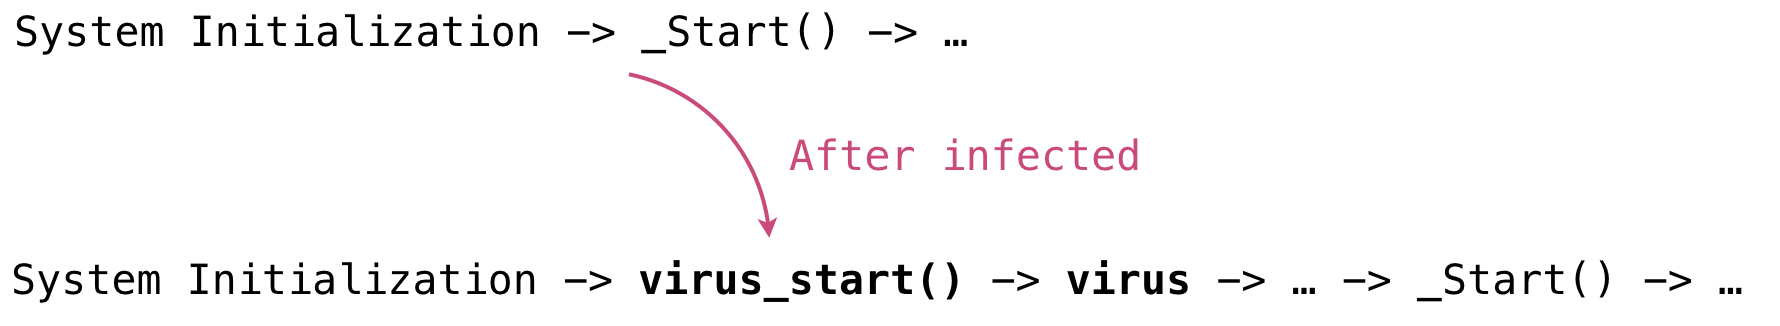
\includegraphics[width = \textwidth]{figures/fig1_order}
		\caption{静态链接病毒}
		\label{fig:way1}
	\end{figure*}
然而这种做法存在一个比较大的隐患——如果自己与目标程序在地址空间的使用上重叠,那么就无法正常嵌入代码。
\subsection{PIE:位置无关可执行文件}
若病毒体使用位置相关代码,在宿主地址空间从\texttt{0x400000}到\texttt{0x800000}被占用的情况下,病毒体就无法使用\texttt{0x400000}和\texttt{0x800000}之间的地址。虽然我们可以通过修改链接器使用脚本来控制病毒代码的链接起点,但是静态链接后的结果是不能修改的。因此病毒在感染的时候不可避免的会遇到某些地址空间使用情况重叠的目标程序。为了保证我们的病毒可以有良好的适应性,病毒代码应该是位置无关的,因为它无法知道留给它的地址空间是什么样的。

因此我们想到把我们的代码实现成Position Independent Executable (PIE)\footnote{GCC编译指令\texttt{-fPIE},链接指令\texttt{-pie}}。但是在GCC的链接选项中,PIE和static是冲突的,即PIE程序一定是动态链接,这样一来就造成了一些麻烦。我们尝试了用一个程序把一个PIE-ELF文件的地址空间布局向后偏移0x200000的位置。但如果只是修改Segments的信息是不够的,首次的尝试失败了。后面我们查到了使用动态链接的程序在执行的时候回读取DYNAMIC段的信息,里面包含了一些绝对地址的项,然后通过在代码中添加修改相应项的信息的代码,使得偏移之后的代码可以正常执行了!

通过动态链接使我们的代码正常执行后,我们尝试把两个ELF(病毒与宿主文件)连在一起。但这个时候就出现了又一个困难。我们原本以为只需要把Segments的信息拼接起来即可,然而事实却不尽人意。当我们把两个ELF连接到一起之后,发现程序其实无法正常执行,使用readelf读取合并后的ELF文件,获得警告信息(程序中有两个DYNAMIC段)。在阅读了Linux系统关于加载ELF文件部分的代码后得知,Linux只会使用文件中一个DYNAMIC段内的信息。这就意味着,如果我们的病毒是一个PIE的话,它就只能注入到静态连接的代码中,这就大大地缩小了我们病毒的感染范围。


\subsection{使用一个Wrapper}
由于PIE病毒在机制上的缺陷,我们不得不放弃上面一个思路。之后我们做了一个非常简单却十分巧妙的尝试。
	\begin{figure*}[htbp]
		\centering
		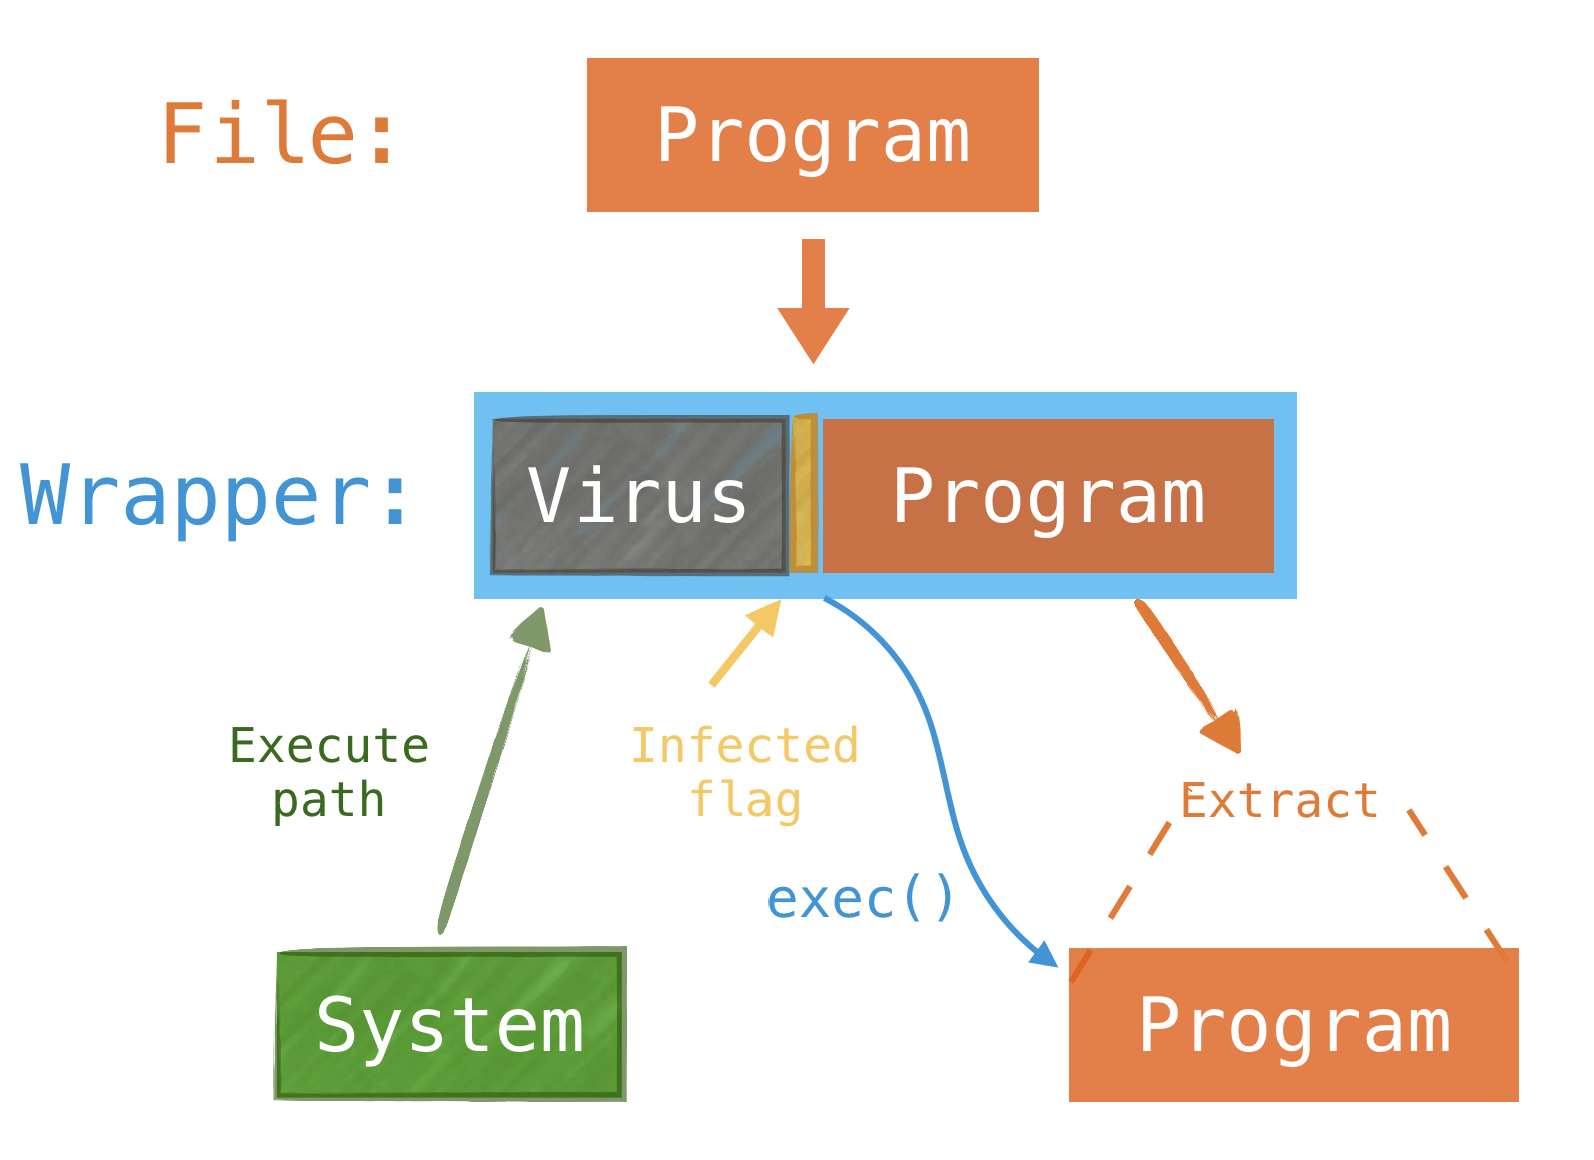
\includegraphics[width = 0.7\textwidth]{figures/fig2_wrapper}
		\caption{用一个Wrapper把宿主文件放在病毒后}
		\label{fig:way3}
	\end{figure*}

如图\ref{fig:way3}所示,我们使用一个Wrapper,把原来的ELF(宿主文件)添加在新的ELF(病毒)的16KB之后的位置,16KB之前的为病毒的ELF文件信息,这样一来,病毒在执行的时候会读取自己16KB之后的文件,然后输出到\texttt{/tmp}目录下面一个文件名随机的文件中,然后再用\texttt{exec}执行宿主程序。

\subsection{终极思路:添加共享库依赖}
\begin{figure}
	\centering
	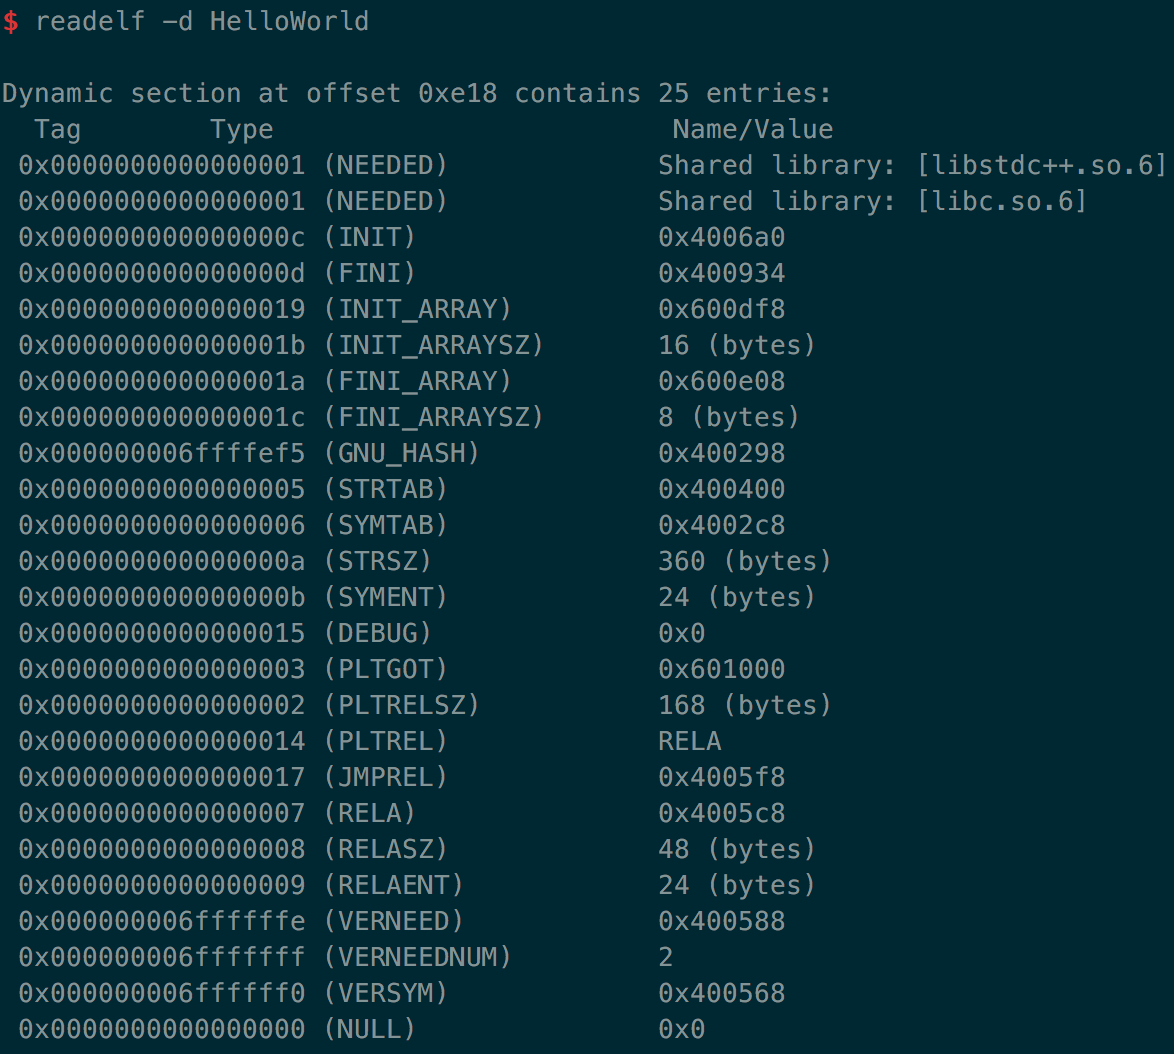
\includegraphics[width=\textwidth]{figures/elf-dynamic-section}
	\caption{一个ELF文件的.dynamic节的信息}
	\label{fig:elf-dynamic}
\end{figure}
由于在尝试平移PIE文件地址空间布局的时候要需要处理DYNAMIC段的信息(图\ref{fig:elf-dynamic}所示),其中包含了对外部共享库依赖信息。因此我们想到,能不能把修改程序的\texttt{DYNAMIC}段的信息,添加一个共享库的依赖,然后把我们的病毒代码放在一个共享库的初始化代码中,这样操作系统在加载被感染的代码的时候就会加载所有被依赖的共享库并且执行共享库的初始化操作(执行病毒代码)。这样只需要对目标ELF作出少量修改即可完成我们的目标。

\begin{figure*}[htbp]
		\centering
		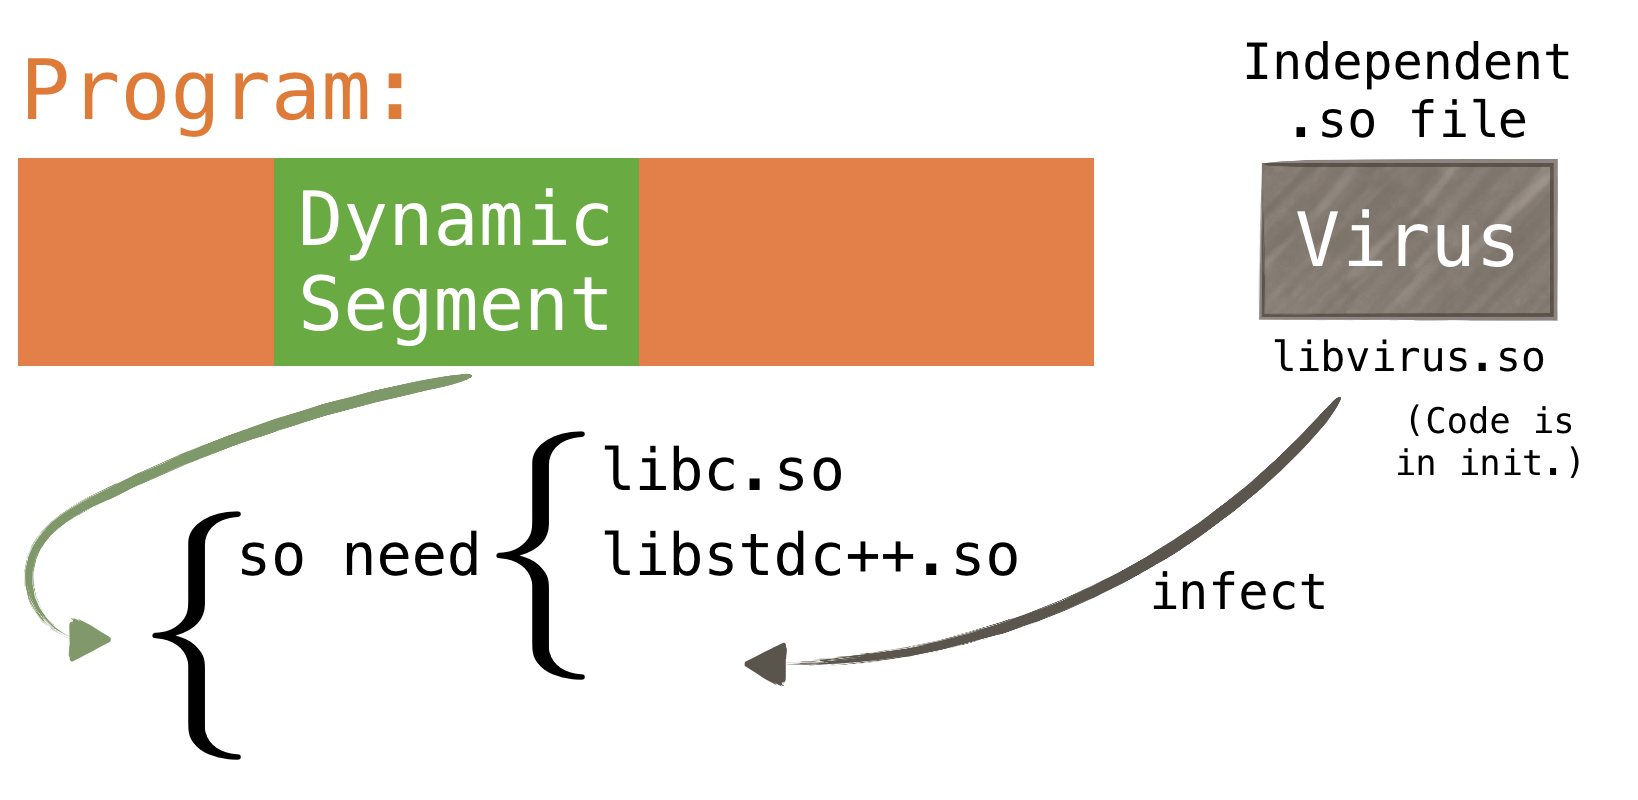
\includegraphics[width =0.7 \textwidth]{figures/fig4_ld1}
		\caption{感染共享库思路示意图}
		\label{fig:way4}
\end{figure*}

由于ELF文件在文件和内存地址空间上的布局是非常紧凑的,要在紧凑的文件中插入一个信息就变得非常繁琐。同时ELF文件本身使用了大量自己定义的结构体,保持了一个树状结构。如果由我们自行编写处理ELF文件的代码,工作量势必变得非常大。因此我们在网络上搜索能够处理ELF文件操作的库时,找到了我们最终使用的ELFIO。这个库用C++编写而成,且只有头文件(虽然在一开始由于C++程序初始化比较复杂的原因,我们决定的是只写C代码,但是由于我们改变了我们感染文件的策略,用C++实现也就变得不是不可以接受了)。 而且一个意外的好处是:这个库并不需要特殊共享库的支持,所有用到的共享库都是Linux系统运行时必须的。这给我们的项目带来了巨大的便利,不需要考虑目标机器上是否有我们需要使用的共享库。


\begin{figure*}[htbp]
		\centering
		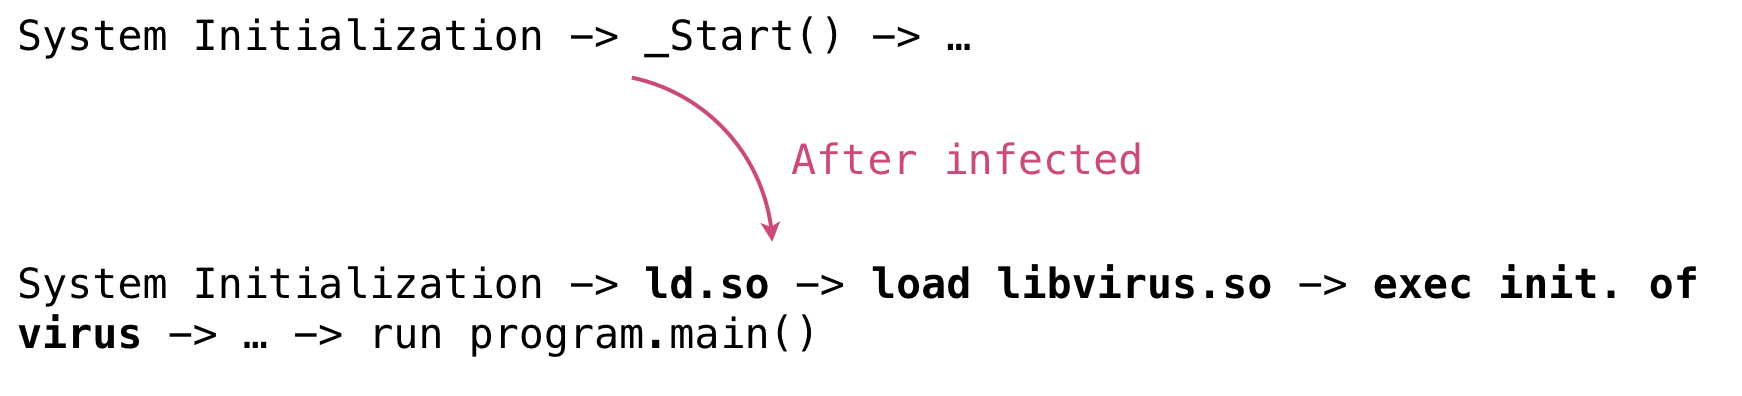
\includegraphics[width = \textwidth]{figures/fig5_ld2}
		\caption{感染前后执行路径对比}
		\label{fig:way4}
\end{figure*}

\section{具体实现}
首先编写病毒部分,把代码编译成共享库\footnote{编译指令\texttt{g++ virus.cc -o libvirus.so -shared -fPIC -...}},然后通过\texttt{dlopen}函数手动加载共享库并成功的执行了写在初始化部分的(C++全局对象的构造函数)病毒代码。这一成功给了我们极大的信心。然后我们开始编写搜索ELF文件中\texttt{.dynstr}和\texttt{.dynamic}信息的代码,然后试图修改并写回文件(在实验中,为了区别感染与未感染,我们感染后的输出并没有直接覆盖源文件)。我们尝试获得了成功。

然后考虑如何包装这个病毒,首先是手动的版本,手动把文件复制到\texttt{/lib/x86\_64-linux-gnu}目录下,然后编写一个调用dlopen函数手动加载so文件的程序激活病毒。后来我们写了一个能够把so文件的内容按字节输出成C的字符串的转义字符(\texttt{\textbackslash xXX},其中XX为该字节的16进制表示),以数据的形式放在一个类似自解压程序中,这个程序在运行的时候会在\texttt{/lib/x86\_64-linux-gnu}目录下创建\texttt{libvirus.so}文件,并且写入正确的信息。然后通过\texttt{dlopen}加载so执行病毒代码。

我们尝试了多线程、多进程感染的支持。我们先把原来单线程的感染操作(在初始化的时候扫描目录,感染文件)改成了多线程。但是因为特殊的原因,单进程多线程的做法并不能满足我们的要求。最后我们使用了多进程的方法来实现不阻塞的感染。幸运的是,由于我们是一个so文件,调用fork之后通过ps查看到的只是原程序的路径,这样可以欺骗用户是他们用特殊方法执行了两次程序。
\subsection{具体实现}
实现的思路非常简单,第一步尝试在\texttt{.dynstr}节中增加一个字符串,该字符串的内容为病毒共享库的名字。然后在\texttt{.dynamic}节中找到类型为\texttt{DT\_NULL}的项目,改成\texttt{DT\_NEED},并且处理数据值。
\subsubsection{增加新Section}
由于在ELF文件中\texttt{.dynstr}之后紧接着就是\texttt{.dynsym}节,并没有足够的空间来放下我们的新字符串。幸运的是,GCC编译生成的代码中,只读内存段和读写内存段之间有\texttt{0x200000}的空间,使得我们可以在只读内存段的最后添加一个新的节,然后把原来的\texttt{.dynstr}中的信息复制一份并且加载我们的新字符串。
\subsubsection{修改.dynamic节中描述字符串表位置的项}
在.dynamic节中类型为\texttt{DT\_STRTAB}的项记录了动态链接使用的字符串表在文件中的位置,\texttt{DT\_STRSZ}项记录了该字符串表的大小。只需要把这两个项的手修改正确即可。
\subsubsection{在.dynamic中增加一个项}
一般而言,GCC编译生成的\texttt{DYNAMIC}段会包含30个项,但是实际一般用到的不过是27个项左右,剩下的项均以\texttt{DT\_NULL}的类型填充,操作系统在读取信息的时候也会忽略第一个\texttt{DT\_NULL}项之后的信息。因此我们只需要找到第一个\texttt{DT\_NULL}项,把类型改为\texttt{DT\_NEEDED},同时把数据值改为共享库名字在\texttt{.dynstr}中的偏移即可
\section{小结}
	我们在本次大作业中设计了一个可以感染ELF文件的病毒。经过诸多尝试后,我们确定了以用共享库为感染源的设计思路。我们将病毒代码放在一个共享库的初始化代码中。感染时,病毒会改变程序\texttt{DYNAMIC}段的信息,添加一个共享库的依赖,如此当操作系统加载被感染代码时,就会加载被依赖的共享库并执行初始化操作,即执行我们的病毒代码。这样的设计有许多好处:1)轻量级,只需修改ELF少量内容即可达成目标;2)隐蔽性,由于是一个病毒是一个so文件,ps查看到的只是原程序路行,用户会以为是自己执行了两次程序。并且用户在排查可执行文件时不会发现任何问题;3)扩展性,我们病毒不仅可以感染可执行文件,而且可以感染所有object文件。这种感染方式不需要用户执行被感染母体,甚至在执行未被感染文件时都可能触发病毒代码。以上就是我们ELF病毒的全部内容,我们在github上公开了代码\footnote{代码地址:\url{https://github.com/BreakVoid/badkid}} , 希望能给读者朋友带来一些帮助。
\end{document}
